\documentclass[12pt]{report}
\usepackage{amsmath}
\usepackage{latexsym}
\usepackage{amsfonts}
\usepackage[normalem]{ulem}
\usepackage{soul}
\usepackage{array}
\usepackage{amssymb}
\usepackage{extarrows}
\usepackage{graphicx}
\usepackage[backend=biber,
style=numeric,
sorting=none,
isbn=false,
doi=false,
url=false,
]{biblatex}\addbibresource{bibliography-biblatex.bib}

\usepackage{subfig}
\usepackage{wrapfig}
\usepackage{wasysym}
\usepackage{enumitem}
\usepackage{adjustbox}
\usepackage{ragged2e}
\usepackage[svgnames,table]{xcolor}
\usepackage{tikz}
\usepackage{longtable}
\usepackage{changepage}
\usepackage{setspace}
\usepackage{hhline}
\usepackage{multicol}
\usepackage{tabto}
\usepackage{float}
\usepackage{multirow}
\usepackage{makecell}
\usepackage{fancyhdr}
\usepackage[toc,page]{appendix}
\usepackage[hidelinks]{hyperref}
\usetikzlibrary{shapes.symbols,shapes.geometric,shadows,arrows.meta}
\tikzset{>={Latex[width=1.5mm,length=2mm]}}
\usepackage{flowchart}\usepackage[paperheight=11.69in,paperwidth=8.27in]{geometry}
\usepackage[utf8]{inputenc}
\usepackage[T1]{fontenc}
\TabPositions{0.49in,0.98in,1.47in,1.96in,2.45in,2.94in,3.43in,3.92in,4.41in,4.9in,5.39in,5.88in,}

\urlstyle{same}

\renewcommand{\_}{\kern-1.5pt\textunderscore\kern-1.5pt}

\setcounter{tocdepth}{5}
\setcounter{secnumdepth}{5}

\setlistdepth{9}
\renewlist{enumerate}{enumerate}{9}
		\setlist[enumerate,1]{label=\arabic*)}
		\setlist[enumerate,2]{label=\alph*)}
		\setlist[enumerate,3]{label=(\roman*)}
		\setlist[enumerate,4]{label=(\arabic*)}
		\setlist[enumerate,5]{label=(\Alph*)}
		\setlist[enumerate,6]{label=(\Roman*)}
		\setlist[enumerate,7]{label=\arabic*}
		\setlist[enumerate,8]{label=\alph*}
		\setlist[enumerate,9]{label=\roman*}

\renewlist{itemize}{itemize}{9}
		\setlist[itemize]{label=$\cdot$}
		\setlist[itemize,1]{label=\textbullet}
		\setlist[itemize,2]{label=$\circ$}
		\setlist[itemize,3]{label=$\ast$}
		\setlist[itemize,4]{label=$\dagger$}
		\setlist[itemize,5]{label=$\triangleright$}
		\setlist[itemize,6]{label=$\bigstar$}
		\setlist[itemize,7]{label=$\blacklozenge$}
		\setlist[itemize,8]{label=$\prime$}

\setlength{\topsep}{0pt}\setlength{\parskip}{8.04pt}
\setlength{\parindent}{0pt}

\renewcommand{\arraystretch}{1.3}


\begin{document}

\vspace{\baselineskip}

\vspace{\baselineskip}

\vspace{\baselineskip}
\begin{Center}
{\fontsize{24pt}{28.8pt}\selectfont \textbf{CSE 344}}
\end{Center}
\begin{Center}
{\fontsize{24pt}{28.8pt}\selectfont \textbf{SYSTEMS PROGRAMMING}}
\end{Center}
\begin{Center}
{\fontsize{24pt}{28.8pt}\selectfont \textbf{SPRING 2021}}
\end{Center}

\vspace{\baselineskip}
\begin{Center}
{\fontsize{24pt}{28.8pt}\selectfont \textbf{MIDTERM HOMEWORK}}
\end{Center}
\begin{Center}
{\fontsize{24pt}{28.8pt}\selectfont \textbf{REPORT}}
\end{Center}

\vspace{\baselineskip}
\begin{Center}
{\fontsize{24pt}{28.8pt}\selectfont \textbf{TURKER TERCAN}}
\end{Center}
\begin{Center}
{\fontsize{24pt}{28.8pt}\selectfont \textbf{171044032}}
\end{Center}

\vspace{\baselineskip}

\vspace{\baselineskip}

\vspace{\baselineskip}

\vspace{\baselineskip}
\begin{justify}
{\fontsize{16pt}{19.2pt}\selectfont \uline{HOMEWORK’S CHALLANGE:}}
\end{justify}
\begin{itemize}
	\item Trying to solve complex producer and consumer problem with maximum 7 semaphores.
	\item Free to use anything we have learnt up to now.
	\item We’re going to emulate a covid –19 vaccination processes.
	\item Our input file will contain enough vaccines for both first and second vaccine shots.
	\item Nurses will read the input file by 1 character at a time, and it’ll write it to a shared buffer.
	\item Vaccinators will consume the buffer by taking a first vaccine and a second vaccine at a single time and then, it will communicate with oldest registered citizen.
	\item If a citizen gets both 1\textsuperscript{st} and 2\textsuperscript{nd} shots t times, citizen terminates.
	\item If all the citizens terminate, program finishes successfully.
\end{itemize}

\vspace{\baselineskip}

\vspace{\baselineskip}
\begin{justify}
{\fontsize{16pt}{19.2pt}\selectfont \uline{DESIGN CHOICES:}}
\end{justify}
\begin{justify}
{\fontsize{14pt}{16.8pt}\selectfont \uline{Communication and Synchronization:}}
\end{justify}
\begin{itemize}
	\item 7 different semaphores
\setlength{\parskip}{0.0pt}
\begin{itemize}
	\item Empty Semaphore: To check if the buffer size is full. If it is full don’t let any Nurses to write to buffer.

\vspace{\baselineskip}
	\item Full Semaphore: To check if the buffer size is empty. If it is empty don’t let any Vaccinators to consume any item from the buffer.

\vspace{\baselineskip}
	\item First Vaccine Semaphore: It contains number of 1\textsuperscript{st} vaccines in the buffer.If buffer is not containing any 1\textsuperscript{st} vaccine, don’t let any Vaccinator to continue. It will need both 1\textsuperscript{st} and 2\textsuperscript{nd}.

\vspace{\baselineskip}
	\item Second Vaccine Semaphore: It works like first vaccine semaphore. Only difference is it contains number of 2\textsuperscript{nd} vaccines.

\vspace{\baselineskip}
	\item Mutex – 1: In order to protect critical region shared between Nurses and Vaccinators. Only one of them can consume or produce item at a time.

\vspace{\baselineskip}
	\item Mutex – 2: I used shared memory segments to store citizen’s pid, how many shots it needs and if it is receiving a shot at the moment. So, to protect this shared memory segment between Vaccinators and don’t letting them to vaccinate same person, I used a mutex.

\vspace{\baselineskip}
	\item Ready to go Semaphore: Each Nurse, Vaccinator and Citizen processes starts differently. If the Citizen size is large, there is chance that a citizen may finish before all the Vaccinators start. This condition is a race condition at causes a deadlock because I created for each Citizen a fifo to communicate between the Vaccinators and itself. So, if it finishes before every other Vaccinator opens its fifo, Fifo would not have any reading end. So, every Vaccinator would be blocked forever. Each Nurse, Vaccinator and Citizen process, after necessary implementation like open up to shared memory etc., it will write to Clinics fifo. After all the writing is done, clinic will raise this semaphore.

\vspace{\baselineskip}

\end{itemize}
	\item SIGINT and SIGUSR1 signals
\begin{itemize}
	\item SIGINT: I saved all the Nurse, Vaccinator and Citizen’s pids in the arrays. If a CTRL + C signal (SIGINT) arrives, Client sends SIGINT signal to all the child processes it has, then, they terminate immediately. 
	\item SIGUSR1: After all the Citizens have received their shots, all the processes should have finished. So, if all Citizens terminate, Clinic sends SIGUSR1 signal to Nurses and Vaccinators which means that they should terminate immediately.
\begin{justify}
 
\end{justify}

\end{itemize}
	\item FIFO
\begin{itemize}
	\item I created a fifo for each Citizen to communicate with between Vaccinators. \\
A Vaccinator sends message that it contains how many Vaccine-1 and Vaccine-2 that buffer has and the how many Citizens are remaining to getting shots.
	\item And I created a fifo for the Clinic so that every child can message to Clinic to state that it is ready.
\end{itemize}
\end{itemize}

\vspace{\baselineskip}
\begin{justify}
{\fontsize{14pt}{16.8pt}\selectfont \uline{Shared Memory Segments:}}
\end{justify}
\begin{itemize}
	\item Shared File Descriptor: I used fork and exec for creating and running different types of processes. After exec, each Nurse must share a common file descriptor for reading from the input file.

\vspace{\baselineskip}
	\item Shared Buffer: I used an integer array that is size is specified in the arguments. Nurses and Vaccinators must share it for the consuming and producing vaccines.

\vspace{\baselineskip}
	\item Shared Buffer Size: While Nurses are producing and Vaccinators consuming, they should have known the shared buffer’s size.
\end{itemize}

\vspace{\baselineskip}
\begin{itemize}
	\item Citizen Array: Vaccinators must know the which citizen is oldest, how many shots it is still waiting for, and it is receving a shot now (If it is busy).
\end{itemize}

\vspace{\baselineskip}

\vspace{\baselineskip}

\vspace{\baselineskip}

\vspace{\baselineskip}
\begin{adjustwidth}{0.5in}{0.0in}
\begin{justify}
Code for this type struct:
\end{justify}
\end{adjustwidth}

\begin{adjustwidth}{0.5in}{0.0in}
\begin{justify}
\tab struct reg\_citizen $ \{ $ 
\end{justify}
\end{adjustwidth}

\begin{adjustwidth}{0.5in}{0.0in}
\begin{justify}
\tab \tab pid\_t pid;
\end{justify}
\end{adjustwidth}

\begin{adjustwidth}{0.5in}{0.0in}
\begin{justify}
\tab \tab int count;
\end{justify}
\end{adjustwidth}

\begin{adjustwidth}{0.5in}{0.0in}
\begin{justify}
\tab \tab int busy\_flag;
\end{justify}
\end{adjustwidth}

\begin{adjustwidth}{0.5in}{0.0in}
\begin{justify}
$ \} $ 
\end{justify}
\end{adjustwidth}

\begin{adjustwidth}{0.49in}{0.0in}
\begin{justify}
When the Clinic is creating Citizen processes, It will store each Citizen’s pid in the array with the increasing order. So that, the oldest process (small pid) should have been get shot first.
\end{justify}
\end{adjustwidth}


\vspace{\baselineskip}
\begin{itemize}
	\item Vaccine Types: I indicated that I used for semaphores for how many 1\textsuperscript{st} and 2\textsuperscript{nd} vaccine we had but, since it’s a semaphore’s value is not always correct. Since Vaccinators may hold the semaphore value. So. I created shared memory for storing how many 1\textsuperscript{st} and 2\textsuperscript{nd} vaccines we had and printing them correctly.
\end{itemize}

\vspace{\baselineskip}

\vspace{\baselineskip}
\setlength{\parskip}{8.04pt}
\newpage
\begin{justify}
{\fontsize{16pt}{19.2pt}\selectfont \uline{clinic.c}}
\end{justify}
\begin{itemize}
	\item Program starts with the clinic. It handles and manages resources, initializations of Nurses, Citizens, Vaccinators, initializes semaphores, fifos and shared memory segments.

\vspace{\baselineskip}
	\item First it checks the arguments are valid or not by looking at below conditions.
\end{itemize}
\begin{adjustwidth}{0.5in}{0.0in}
\begin{justify}
n >= 2: the number of nurses (integer)
\end{justify}
\end{adjustwidth}

\begin{adjustwidth}{0.5in}{0.0in}
\begin{justify}
v >= 2: the number of vaccinators (integer)
\end{justify}
\end{adjustwidth}

\begin{adjustwidth}{0.5in}{0.0in}
\begin{justify}
c >= 3: the number of citizens (integer)
\end{justify}
\end{adjustwidth}

\begin{adjustwidth}{0.5in}{0.0in}
\begin{justify}
b >= tc+1: size of the buffer (integer),
\end{justify}
\end{adjustwidth}

\begin{adjustwidth}{0.5in}{0.0in}
\begin{justify}
t >= 1: how many times each citizen must receive the 2 shots (integer),
\end{justify}
\end{adjustwidth}

\begin{adjustwidth}{0.5in}{0.0in}
\begin{justify}
i: pathname of the input file
\end{justify}
\end{adjustwidth}

\begin{itemize}
	\item It creates a fifo for each Citizen with this template. 
\begin{itemize}
	\item /tmp/process\_pid

\vspace{\baselineskip}

\end{itemize}
	\item And then, it forks and execs for Nurse, Citizen and Vaccinator processes. For the further use of the child processes, it sends necessary arguments for them.
\end{itemize}

\vspace{\baselineskip}

\vspace{\baselineskip}
\begin{itemize}
	\item Then it waits for all the child processes to terminate or a SIGINT signal. If SIGINT arrives, it sends SIGINT signal to all children processes. If all the Citizen processes have been terminated, It sends SIGUSR1 signal for Nurse and Vaccinators and then, they will be terminated too. And after that it closes all the managed resources, semaphores, etc. And the program ends.
\end{itemize}

\vspace{\baselineskip}
\newpage
\begin{justify}
{\fontsize{16pt}{19.2pt}\selectfont \uline{nurse.c}}
\end{justify}
\begin{itemize}
	\item Nurse is very similar to classic\ producer.  Only difference is the is increments the semaphore for the First and Second Vaccine Semaphore according to which vaccine it produces. 
	\item And it has a a signal handler for both SIGINT and SIGUSR1.
\end{itemize}
\begin{justify}
{\fontsize{16pt}{19.2pt}\selectfont \uline{vaccinator.c}}
\end{justify}
\begin{itemize}
	\item I divided the code to two parts. First part is the consume from the buffer both 1\textsuperscript{st} and 2\textsuperscript{nd} vaccine and I used first semaphore for this critical region. 
	\item Second part is selecting oldest person in the shared citizen array. And it sends a message via chosen’s FIFO and makes the boolean value for the chosen person 1 and that means that it is busy right now. While the chosen is busy, no other vaccinators cannot choose it. After the message is sent, vaccinator sets 0 to busy part and decrements the count of how many vaccines the chosen citizen gets by 1.
\end{itemize}
\begin{justify}
{\fontsize{16pt}{19.2pt}\selectfont \uline{citizen.c}}
\end{justify}
\begin{itemize}
	\item It waits for the message from its fifo. 
	\item After message arrives, it prints the message that it got shot for the which time and how many vaccines the buffer has.
	\item If it got all the shots that is needed, it terminates.
\end{itemize}

\vspace{\baselineskip}

\vspace{\baselineskip}

\vspace{\baselineskip}

\vspace{\baselineskip}

\vspace{\baselineskip}

\vspace{\baselineskip}

\vspace{\baselineskip}

\vspace{\baselineskip}

\vspace{\baselineskip}
\newpage
\begin{justify}
{\fontsize{16pt}{19.2pt}\selectfont \uline{TESTS AND VALGRIND:}}
\end{justify}
\begin{justify}
I tried some many tests for this program. Since the outputs of the program is large, I saved this test cases in the below .txt files
\end{justify}
\begin{justify}
Test 1: 
\end{justify}
\begin{justify}
> log\_4c\_2t.txt
\end{justify}


\begin{figure}[H]
	\begin{Center}
		
\includegraphics[width=6.54in,height=0.61in]{image1.png}
	\end{Center}
\end{figure}




\vspace{\baselineskip}\begin{justify}
Test 2:
\end{justify}
\begin{justify}
> valgrind\_log\_4c\_2t.txt
\end{justify}


\begin{figure}[H]
	\begin{Center}
		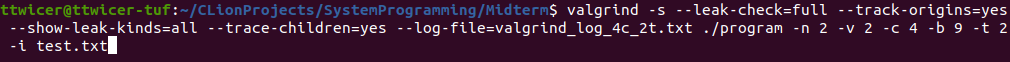
\includegraphics[width=6.57in,height=0.4in]{image2.png}
	\end{Center}
\end{figure}




\vspace{\baselineskip}\begin{justify}
Test 3:
\end{justify}
\begin{justify}
> log\_8c\_4t.txt
\end{justify}


\begin{figure}[H]
	\begin{Center}
		
\includegraphics[width=5.0in,height=0.22in]{image3.png}
	\end{Center}
\end{figure}



\vspace{\baselineskip}
\vspace{\baselineskip}
\begin{justify}
Test 4:
\end{justify}
\begin{justify}
> log\_32c\_4t.txt
\end{justify}


\begin{figure}[H]
	\begin{Center}
		
\includegraphics[width=5.0in,height=0.23in]{image4.png}
	\end{Center}
\end{figure}



\vspace{\baselineskip}
\vspace{\baselineskip}
\begin{justify}
Test 5:
\end{justify}
\begin{justify}
> log\_64c\_8t.txt
\end{justify}


\begin{figure}[H]
	\begin{Center}
		
\includegraphics[width=5.0in,height=0.16in]{image5.png}
	\end{Center}
\end{figure}



\vspace{\baselineskip}
\vspace{\baselineskip}
\begin{justify}
Test 6:
\end{justify}
\begin{justify}
> log\_256c\_8t.txt
\end{justify}


\begin{figure}[H]
	\begin{Center}
		
\includegraphics[width=5.0in,height=0.15in]{image6.png}
	\end{Center}
\end{figure}



\vspace{\baselineskip}
\vspace{\baselineskip}
\begin{justify}
Test 7:
\end{justify}
\begin{justify}
> log\_512c\_64t.txt
\end{justify}

\begin{figure}[H]
	\begin{Center}
		
\includegraphics[width=5.0in,height=0.18in]{image7.png}
	\end{Center}
\end{figure}



\vspace{\baselineskip}
\vspace{\baselineskip}
\begin{justify}
{\fontsize{16pt}{19.2pt}\selectfont \uline{Final Notes:}}
\end{justify}
\begin{itemize}
	\item I tried some many times for these tests and none of them is failed with a input that has 2 $\ast$  t $\ast$ c vaccines. And I also tried it above tests some many times with my bash script it worked perfect too. But if a deadlock happens. Please kill the program with CTRL + C signal and run again.
	\item I completed the optional bonus part.
\end{itemize}
\begin{itemize}
	\item I think I adhered to every constraint you stated in the assignment and every attribute you specified.
	\item The only problem that I couldn’t solve was if the number of the citizens is larger than 1024, the citizens that is created after that 1024\textsuperscript{th} citizen, their fifos doesn’t work. I guess the limit how many fifos a program create is 1024.
\end{itemize}
\printbibliography
\end{document}